%\documentclass[onecolumn]{IEEEtran}
\documentclass{article}
\usepackage[nonatbib]{neurips_2020}
%\usepackage{natbib}
\usepackage[utf8]{inputenc}

\usepackage{IEEEtrantools}
%\usepackage{standalone}
%\include{examplepreamble}
%\standaloneconfig{}
%\usepackage[subpreambles=true]{standalone}
\usepackage{import}
\usepackage{framed}

%\usepackage[hidelinks]{hyperref}

%\usepackage{cite}

\usepackage{caption}
%\usepackage{graphicx}
%\usepackage{float}
%\usepackage{listing}
\usepackage[dvipsnames]{xcolor}
\definecolor{LGray}{gray}{0.98}
\definecolor{dgray}{gray}{0.3}
\usepackage{scrextend}
\usepackage{hyperref}
\hypersetup{
	colorlinks=true,
	linkcolor=blue,
	filecolor=magenta,      
	urlcolor=cyan,
	citecolor=dgray,
}



%%% for code wraping
\usepackage{minted}
\usemintedstyle{colorful}
\setminted[julia]{frame=lines,rulecolor=MidnightBlue,bgcolor=LGray,fontsize=\footnotesize ,breaklines}
\usepackage{tikz}
\usetikzlibrary{shapes.geometric, arrows}
\usetikzlibrary{mindmap}

\tikzstyle{layer} = [rectangle, rounded corners, minimum width=3cm, minimum height=1cm,text centered, draw=black]
\tikzstyle{arrow} = [thick,->,>=stealth]


\usepackage{pmboxdraw}
%\usepackage{qtree}
%\usepackage{subcaption}


\usepackage{array}
\usepackage{multirow}

\title{NumNN.jl: A Toolkit for Simulating Deeplearning Networks Supporting on Non-Conventional Arithmetic}

\author{%\IEEEauthorblockN
	{Mohammad~Hizzani}\\
	%\IEEEauthorblockA
	%{
	INESC-ID\\ 
	Instituto Superior Técnico\\ 
		Universidade de Lisboa\\
		Email: \href{mailto:moh.hizzani@gmail.com}{\tt moh.hizzani@gmail.com}%}
	\And
	%\IEEEauthorblockN
	{Leonel Sousa}\\
	%\IEEEauthorblockA
	%{
	INESC-ID\\ 
		Instituto Superior Técnico\\ 
		Universidade de Lisboa\\
		Email: \href{mailto:las@inesc-id.pt}{\tt las@inesc-id.pt}%}
	%Email: some@sdf.com}
}


\begin{document}
	\maketitle

	\begin{abstract}
		The development of Deeplearning models requires hardware support, with deep architectures (organized around different number of layers and computations per layer whether they are nodes of fully-connected layers or channels of convolutional neural networks). Moreover, deeplearning models use big data for training, with the need for tuning the hyper parameters, requiring the repetition of the whole training process multiple times. Thus, hardware-friendly number systems and arithmetic have been introduced alternatively to the IEEE floating-point formats, which are cost effective and/or more accurate. However, the hardware design, verification and assessment are more complex and expensive processes. Hence, these arithmetic systems should be tested in simulation environments for the target applications, before moving forward to system design. Since most deeplearning frameworks and libraries target AI production, they only support the IEEE formats. This paper presents NumNN.jl, a tool for supporting and facilitating the design and prototyping of deeplearning systems based on different number representations. It provides an agile way of designing, training and evaluating any type of deeplearning (neural network) model with any number and arithmetic system(s).
	\end{abstract}

	\section{Introduction}

%\IEEEPARstart{M}{any}
Many new and old number systems have been introduced as an alternative to IEEE-754 standards \cite{754} for deeplearning. Some of them have been used in many different fields of Digital Signal Processing (DSP) and other specific applications, namely for and to process several types of neural networks (i.e. Fully-connected layers, CNN and RNN).

\subsection{Examples of Number Systems For Deeplearning}

An example of a non-conventional number systems is the Posit number system, which is known also as UNUM III \cite{Gustafson2017}. Posit was introduced as an advanced number system that overpasses IEEE standards as a hardware-friendly system for general-purpose arithmetic. It also provides faster versions of functions used in neural networks such as the sigmoid function\footnote{Sigmoid function $\left(\sigma(x) = \frac{1}{1 + e^{-1}}\right)$ is an activation function, the $\tanh$ function is widely used and it is a scaled and shifted version of the Sigmoid function $\left(\tanh(x) = 2 \sigma(2x) -1\right)$.}.

Some suggested number systems can be modified to perform faster computation than the conventional IEEE-754 such as Logarithmic Number Systems (LNS) \cite{Kingsbury1971} and Residual Number System (RNS) \cite{Garner1959}. The RNS has been being used in many DSP applications \cite{Cardarilli2007,Chaves2003,Claudio1995,DiClaudio1990,Jullien1987} and other extensive computational applications like asymmetric (public-key) cryptography \cite{Sousa2016}. RNS was used to provide energy-saving units in Convolution Neural Networks (CNN) \cite{Samimi2020}.

LNS \cite{Kingsbury1971,Alexopoulos1975,Lee1977} has also been used in many applications including DSP \cite{Dimitrov2001,Lewis1995}. Recently it has been developed to be used in CNN, in order to provide high accuracy in training using significantly smaller bit length \cite{Miyashita2016,Juang2019}.

\subsection{Why The Julia Programming Language}

Julia \cite{Julia,Bezanson2017} is a high-level programming language that was designed for numerical and scientific computation, well suited for data science. It provides an unconventional way of defining primitive types at hardware level (with number of bits predefined), where all data types of Julia defined, designed and implemented using only native Julia\footnote{\mintinline{julia}{Float16, Float32, Float64} represent the IEEE Floating types in Julia. \mintinline{julia}{Int128, Int16, Int32, Int64, Int8} are the conventional Signed-Integers similarly \mintinline{julia}{UInt128, UInt16, UInt32, UInt64, UInt8} are the conventional Unsigned integers.}.

Moreover, Julia provides a novel way of handling \emph{multiple dispatch} \cite{WikiMultipleDispatch} concept in programming languages \cite{JuliaMehtods}. Multiple Dispatch in a nutshell is that a function with a single name has different processes (methods) base on its argument(s). Examples of multiple dispatch are the primitive operations (addition, subtraction, multiplication and division) as follows:

\begin{listing}[H]
\begin{minted}{julia}
julia> aInt, bInt = 1, 2; #these are Integers

julia> aF, bF = 1.0, 2.0; #there are Floats

julia> aInt + bF #this will call the method +(::Integer, ::Float64) note the result is in Float64
3.0
\end{minted}
\caption{Multiple Dispatch Example}
\end{listing}

Note how the result was promoted to be in \mintinline{julia}{Float64} because of Julia special promotion functions (\mintinline[fontsize=\footnotesize ]{julia}{promote_type(::Type{Integer},::Type{Float64}) = Float64}). This means that functions used in any package can be used without making any modification to the package, it is only required to define methods of those functions for the new type. For instance, functions such as trigonometric functions or hyperbolic functions as by default provided by Julia for its primitive types including the IEEE-754. If any of these exists in a package simply define any of them for the new number system that is to be used in this package, further details will be given in subsection~\ref{subsec:saa}.

\textbf{Divide and conquer} is an essential approach of development, which facilitates the focus on smaller pieces of a development process by dividing a system into layers, each layer is easily analyzed and improved. Hence, this property of Julia (Multiple Dispatch) makes it easier to separate different steps, and then integration with it is a separated process. This means that less time is used on editing and modifying, and more time is used for designing, testing and developing. The upcoming sections will present the methods of functions of NumNN.jl with which any new number system should be defined beforehand.

Furthermore, Julia provides a native support for parallel operations, namely co-routines, multi-threads and multi-core. Mostly, no new code is needed for parallel operations, the same code with some macros can be used to process in parallel. In the same way, for-loops in Julia are as fast as for-loops in C programming language. 

	
	\section{Structure and Organization}

The NumNN.jl  package\footnote{The Software Toolkit presented in this paper will be made available when paper is accepted}% \url{https://github.com/MohHizzani/NumNN.jl}} 
 (library) was built on the concept of Rapid Prototyping to enable fast experimentation. \emph{Begin able to go from idea to result with the least possible delay is key to good research} \cite{Keras}. There are many deeplearning frameworks \cite{Abadi2016,Collet2015,Jia2014,Paszke2017,PyTorch2019}, some widely spread and efficient in production and research as long as IEEE-754 representation in adopted. However, most of these libraries run on Python with no native support for newly added primitive types nor the efficiency of Julia in multiple dispatch (i.e. any number system needs an internal modification to the library itself to be capable of handling it). Even packages of Julia like Flux.jl \cite{Flux.jl-2018,Innes2018} or Knet \cite{Yuret2016k} neither of them fully support newly added types, and do not provide the flexibility of different types for different parameters or to deliver output with certain desired data types. While NumNN.jl provides a fully support for a total in one type computation, and the ability to choose the type of each group of parameters and the capabilities of delivering output at any chosen type.

\subsection{Fast Implementation and Deployment}

NumNN.jl provides the fastest possible way to implement a neural network model, train and use it for prediction and testing. Installing the package and using it can be done from a Julia REPL as follows:

\begin{listing}[H]
	\begin{minted}{julia}
	julia> ] add NumNN
	julia> using NumNN
	\end{minted}
	\caption{Adding NumNN.jl and import it}\label{addimport}
\end{listing}

Defining layers sequence can be easily done either like this:

\begin{listing}[H]
	\begin{minted}{julia}
	X_Input, X_Ouput = chain(X_train,[Flatten(),FCLayer(120,:relu),FCLayer(10,:softmax)])
	\end{minted}
	\caption{Chained Layers with no side branch(es)}\label{chain}
\end{listing}


where \mintinline[fontsize=\footnotesize]{julia}{X_train} is the train array or the size of train array. In the case there are some side branches, it can be easily performed as in the example of Inception Net \cite{Szegedy2016} (Listing~\ref{chain} as Figure~\ref{fig:inc} shows what happens in the first 3 lines of Listing~\ref{chain}. \mintinline{julia}{X_Input} is being fed into 5 different layers at the same time and the output of these layers are concatenated using \mintinline{julia}{ConcatLayer} to be fed into the next layer). 

%A group of examples can be found in Appendices.

\subsection{Structure and Architecture}\label{subsec:saa}

The structure of NumNN.jl is simple enough to comprehend and start to amending new elements when require. \figurename~\ref{fig:layerstruct} shows the Layers hierarchy in NumNN.jl, this structure was built to facilitate the use and the future development of NumNN.jl.

The convention of data shape to be used is (data dimension(s), channels, batch size). For instance, when using MNIST \cite{LeCun1998,LeCun1998a} data set, the shape of training data will be (28,28,1,60000), where the first two dimensions are the images' dimensions while the third is the number of channels and the last integer expresses the batch size.

\begin{figure}[!ht]
	\centering
	%\begin{subfigure}{0.95\textwidth}
		%\begin{enumerate}
%\qtreecenterfalse
%\item \Tree [.Layer  FCLayer Activation BatchNorm Flatten Input ]

%\item \Tree [.Layer [.MILayer AddLayer ConcatLayer ]]


%\item \Tree [.Layer [.PaddableLayer
%[.ConvLayer Conv1D Conv2D Conv3D ]
%[.PoolLayer
%[.AveragePoolLayer AveragePool1D AveragePool2D AveragePool3d ]
%[.MaxPoolLayer MaxPool1D MaxPool2d MaxPool3d ]]]]
%\end{enumerate}
%\documentclass{article}
%\usepackage{tikz}
%\usetikzlibrary{mindmap}
%\begin{document}


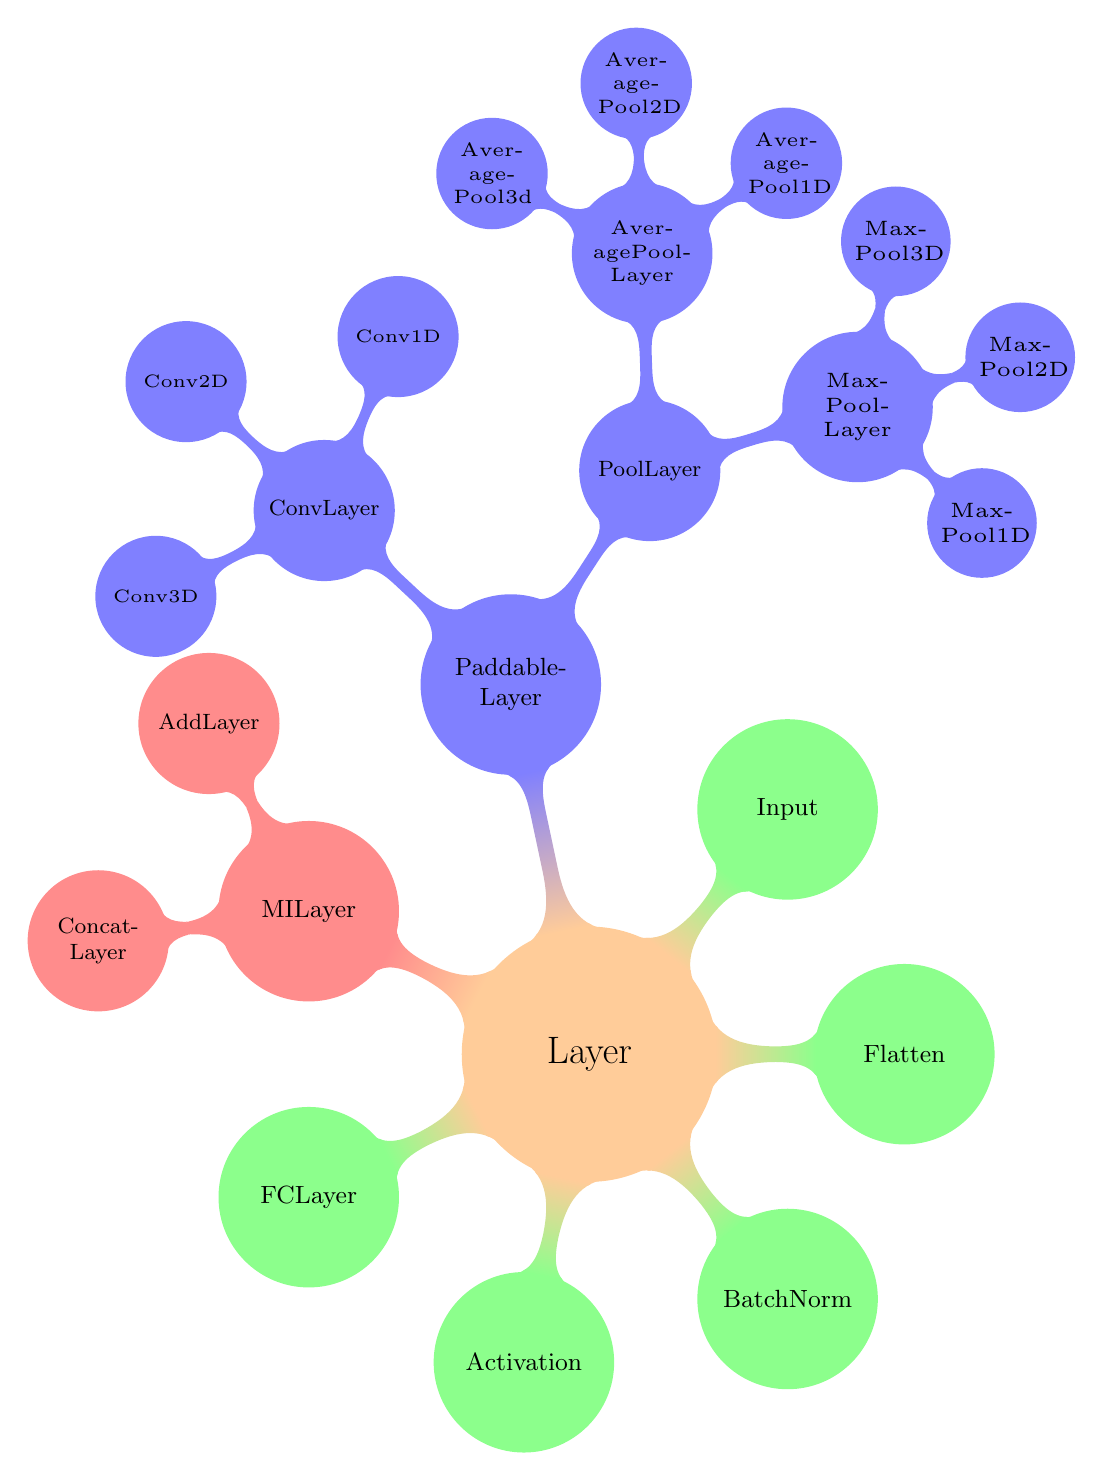
\begin{tikzpicture}[mindmap,
every node/.style={concept,
	execute at begin node=\hskip0pt}, concept color=orange!40,% concept fontsize=10pt,
grow cyclic, %text width=3cm, align=flush center,
level 1/.append style={level distance=4cm,sibling angle=51
},
level 2/.append style={level distance=2.7cm,sibling angle=70
},
level 3/.append style={level distance=2.3cm, sibling angle=70
},
level 4/.append style={level distance=1.8cm,sibling angle=60
}
%,scale=0.6, every node/.style={scale=0.6}
%scale=0.9, transform canvas={scale=0.9}
]
\node[scale=0.8]{\LARGE Layer}
child [concept color=green!45] { node {FCLayer}}
child [concept color=green!45] { node {Activation}}
child [concept color=green!45] { node {BatchNorm}}
child [concept color=green!45] { node {Flatten}}
child [concept color=green!45] { node {Input}}
child [concept color=blue!50, scale=1.2] { node {PaddableLayer}
																	child [sibling angle=90] { node {PoolLayer}
																	child [sibling angle=80] { node [scale=1.5] {MaxPoolLayer}
																		child { node [scale=1.5] {MaxPool1D}}
																		child { node [scale=1.5] {MaxPool2D}}
																		child { node [scale=1.5] {MaxPool3D}}
																	}
																	child { node [scale=1.4] {AveragePoolLayer}
																		child { node [scale=1.4] {AveragePool1D}}
																		child { node [scale=1.4] {AveragePool2D}}
																		child { node [scale=1.4] {AveragePool3d}}
																	}
																}
																child { node {ConvLayer}
																	child [level distance=2cm] { node [scale=1.3] {Conv1D}}
																	child [level distance=2cm] { node [scale=1.3] {Conv2D}}
																	child [level distance=2cm] { node [scale=1.3] {Conv3D}}
															}}
child [concept color=red!45] { node {MILayer}
	child { node {AddLayer}}
	child { node {ConcatLayer}}
			};
\end{tikzpicture}

%\end{document}
	%\end{subfigure}
	\caption{Layer Architecture in NumNN.jl, the useable layers are the leaves the other nodes are \mintinline[fontsize=\footnotesize]{julia}{abstract type}s.}\label{fig:layerstruct}
\end{figure}

An essential data type (\mintinline[fontsize=\footnotesize]{julia}{Model}) holds the main pointers to the layers, structure and parameters to use. Instantiating a (\mintinline[fontsize=\footnotesize]{julia}{Model}) will also invoke the initialization of the layers scaling and bias parameters, which can be done as presented in Listing~\ref{modelinit}.

\begin{listing}[H]
	\begin{minted}{julia}
	model = Model(X_train, Y_train, X_Input, X_Output, 0.001; optimizer=:adam, loss=:categoricalCrossentropy)
	\end{minted}
	\caption{Model initialization, \mintinline{julia}{X_train, Y_train} are training data and labels, while \mintinline{Julia}{X_Input, X_Ouput} are the input and output layers. The value of \mintinline{julia}{0.001} represent the learning rate of this model, where the key-word \mintinline{julia}{optimizer} define the optimizer to be used during training, and \mintinline{julia}{loss} defines the loss function.}\label{modelinit}
\end{listing}

\begin{listing}[!h]
	\begin{minted}{julia}
	X_Input = Input(X_train)
	Xc = [ # use X_Input as an input for these 5 different layers
	Conv2D(3, (3,3), padding=:same)(X_Input),
	Conv2D(4, (5,5), padding=:same)(X_Input),
	Conv2D(10, (1,1), padding=:same)(X_Input),
	MaxPool2D((2,2); padding=:same)(X_Input),
	AveragePool2D((3,3); padding=:same)(X_Input),
	]
	X = ConcatLayer()(Xc) #concatnate the output of all layers in Xc array into one 4D Array
	X = BatchNorm(dim=3)(X) #to normalize across the channels
	X = Activation(:relu)(X)
	X = MaxPool2D((2,2))(X);
	Xc = [ # use X as an input for these 5 different layers
	Conv2D(6, (3,3), padding=:same)(X),
	Conv2D(8, (5,5), padding=:same)(X),
	Conv2D(10, (1,1), padding=:same)(X),
	MaxPool2D((2,2); padding=:same)(X),
	AveragePool2D((3,3); padding=:same)(X),
	]
	X = ConcatLayer()(Xc) #concatnate the output of all layers in Xc array into one 4D Array
	X = BatchNorm(dim=3)(X) #to normalize across the channels
	X = Activation(:relu)(X)
	X = AveragePool2D((3,3))(X);
	X = Flatten()(X)
	X_Output = FCLayer(10, :softmax)(X);
	\end{minted}
	\caption{InceptionNet Example, this layer architecture has many side branches.}\label{chain}
\end{listing}

\begin{figure}[!h]
	\centering
	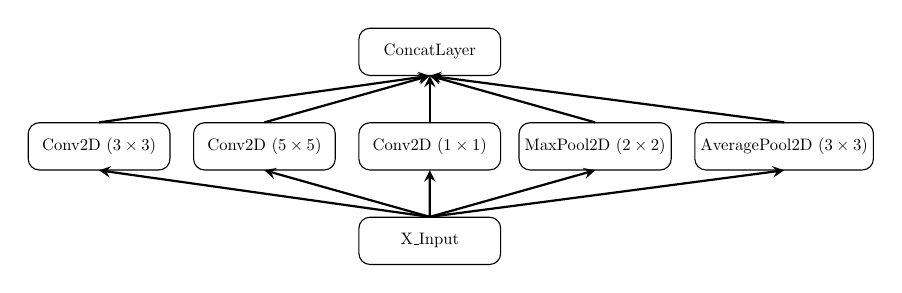
\begin{tikzpicture}[node distance=2cm,scale=0.6, every node/.style={scale=0.6}]
\node (in1) [layer] {X\_Input};
\node (conv1) [layer, above of=in1, xshift=-7cm] {Conv2D $(3\times3)$};
\node (conv2) [layer, right of=conv1, xshift=1.5cm] {Conv2D $(5\times5)$};
\node (conv3) [layer, right of=conv2, xshift=1.5cm] {Conv2D $(1\times1)$};
\node (max1) [layer, right of=conv3, xshift=1.5cm] {MaxPool2D $(2\times2)$};
\node (avg1) [layer, right of=max1, xshift=2cm] {AveragePool2D $(3\times3)$};
\node (concat) [layer, above of=conv3] {ConcatLayer};
\draw [arrow] (in1.north) -- (conv1.south);
\draw [arrow] (in1.north) -- (conv2.south);
\draw [arrow] (in1.north) -- (conv3.south);
\draw [arrow] (in1.north) -- (max1.south);
\draw [arrow] (in1.north) -- (avg1.south);
\draw [arrow] (conv1.north) -- (concat.south);
\draw [arrow] (conv2.north) -- (concat.south);
\draw [arrow] (conv3.north) -- (concat.south);
\draw [arrow] (max1.north) -- (concat.south);
\draw [arrow] (avg1.north) -- (concat.south);
\end{tikzpicture}
	\caption{Listing~\ref{chain} Layers' representation for the first 3 lines}\label{fig:inc}
\end{figure}

Activation functions are defined under the \mintinline[fontsize=\footnotesize]{julia}{abstract type actFun}. NumNN.jl provides a set of activation functions (sigmoid ($\sigma$), \mintinline{julia}{tanh}, \mintinline[fontsize=\footnotesize]{julia}{softmax} and \mintinline[fontsize=\footnotesize]{julia}{noAct}). Any other activation function can be defined as a subtype of \mintinline[fontsize=\footnotesize]{julia}{actFun}, and then as a normal function with another function for its derivative. For instance, $\sin$ has to be added as an activation function, all what is needed is expressed in Listing~\ref{newact}.

\begin{listing}[!ht]
	\begin{minted}{julia}
	abstract type sin <: actFun end
	
	sin(x) = base.sin.(x) #note the use of base. to tell julia that we need the default sin at this step not the type defined because it was overwritten
	dsin(x) = base.cos.(x)
	\end{minted}
	\caption{Example of defining a new activation function to NumNN.jl}\label{newact}
\end{listing}

NumNN.jl has loss functions under the \mintinline{julia}{abstract type lossFun}. The two main loss functions defined are the \mintinline{julia}{binaryCrossentropy} and \mintinline{julia}{categoricalCrossentropy}. Also, other loss functions can be easily defined, more functions will be available in the upcoming versions of NumNN.jl.

%\subsection{Sequence of Processes}
%The easiest way of explaining NumNN.jl is by showing a complete example. 

\subsection{Training, Testing and Evaluating}
To show the effectiveness of NumNN.jl some examples with benchmarks are applied, and accompanied with comparison with another library is presented. Keras on the top of TensorFlow was one of the main influencers upon the syntax of NumNN.jl. Thus, some benchmarks were run on both NumNN and TensorFlow. Nonetheless, some of the benchmarks could not be run on TensorFlow due to lack support for new data types, therefore, they were run only on NumNN.jl.

The data used for train/test was Fashion MNIST \cite{Xiao2017}. Intel(R) Xeon(R) Gold 6140 CPU @ 2.30GHz was used for all tests, and no GPU were used (NumNN does not support GPU and other back-end so far). Table~\ref{tab:bench} shows the results of all test\footnote{%All benchmarks are available at \url{https://github.com/MohHizzani/NumNN.jl/tree/master/examples}
All codes where provided with the paper submit and after acceptance they will be available online}, and where blank is present that means test was not perform under this framework because the data type is not supported\footnote{\label{batchnorm}Benchmark 2 \& 3 has Batch Normalization layer where Float64 is not supported for this layer in TensorFlow}. All benchmarks perform the classification for the Fashion MNIST data using \mintinline{julia}{softmax} as an output layer and \mintinline{julia}{categoricalCrossentropy} as a loss function. Hence, cost is an average of the loss function over all the predicted data, and accuracy was computed as:

\begin{equation}
\textrm{accuracy} = \frac{\textrm{number of correct predictions}}{\textrm{total number of testing labels}}
\end{equation}

\begin{table}[!ht]
	\centering
	\renewcommand{\arraystretch}{1.1}
	\caption{Various benchmarks for NumNN.jl and TensorFlow}\label{tab:bench}
	\begin{tabular}{|c | c | c || c | c |}
		\hline
		Benchmark & DType & Measurements & NumNN.jl & Tensorflow\\\hline\hline
		%%%%%%%%%% Benchmark 1
		\multirow{14}{*}{Benchmark 1} & \multirow{5}{*}{Float32} & Train Accuracy & 0.8902 & 0.9162\\
		& & Test Accuracy & 0.8650 & 0.8851\\
		& & Train Cost & 0.3000 & 0.2270\\
		& & Test Cost & 0.3728 & 0.3444\\
		& & Training Time / Sample & $84\mu$s  & $177\mu$s\\\cline{2-5}
		& \multirow{5}{*}{Float64} & Train Accuracy & 0.8812 & 0.9191 \\
		& & Test Accuracy & 0.8703 & 0.8848 \\
		& & Train Cost & 0.3314 & 0.2163 \\
		& & Test Cost & 0.3845 & 0.3311 \\
		& & Training Time / Sample & $93\mu$s & $100\mu$s\\\cline{2-5}
		& \multirow{4}{*}{Posit\{16,1\}} & Train Accuracy & 0.8716 & \rule{5em}{1pt} \\
		& & Test Accuracy & 0.8510 & \rule{5em}{1pt} \\
		& & Train Cost & 0.3520 & \rule{5em}{1pt} \\
		& & Test Cost & 0.4088 & \rule{5em}{1pt} \\\hline
		%%%%%%%%%% Benchmark 2
		\multirow{14}{*}{Benchmark 2\footref{batchnorm}} & \multirow{5}{*}{Float32} & Train Accuracy & 0.8980 & 0.9160\\
		& & Test Accuracy & 0.8786 & 0.8929\\
		& & Train Cost & 0.2760 & 0.2346\\
		& & Test Cost & 0.3386 & 0.2955\\
		& & Training Time / Sample & $1.31m$s & $8m$s \\\cline{2-5}
		& \multirow{5}{*}{Float64} & Train Accuracy & 0.9020 & \rule{5em}{1pt} \\
		& & Test Accuracy & 0.8857 & \rule{5em}{1pt} \\
		& & Train Cost & 0.2750 & \rule{5em}{1pt} \\
		& & Test Cost & 0.3420 & \rule{5em}{1pt} \\
		& & Training Time / Sample & $1.34m$s & \rule{5em}{1pt} \\\cline{2-5}
		& \multirow{4}{*}{Posit\{16,1\}} & Train Accuracy & 0.9114 & \rule{5em}{1pt} \\
		& & Test Accuracy & 0.8949 & \rule{5em}{1pt} \\
		& & Train Cost & 0.2453 & \rule{5em}{1pt} \\
		& & Test Cost & 0.3045 & \rule{5em}{1pt} \\\hline
		%%%%%%%%%% Benchmark 3
		\multirow{14}{*}{Benchmark 3\footref{batchnorm}} & \multirow{5}{*}{Float32} & Train Accuracy & 0.9136 & 0.9072\\
		& & Test Accuracy & 0.8953 & 0.8899\\
		& & Train Cost & 0.2362 & 0.2527\\
		& & Test Cost & 0.2962 & 0.3050\\
		& & Training Time / Sample & $3.09m$s & $14m$s\\\cline{2-5}
		& \multirow{5}{*}{Float64} & Train Accuracy & 0.9103 & \rule{5em}{1pt} \\
		& & Test Accuracy & 0.8926 & \rule{5em}{1pt} \\
		& & Train Cost & 0.2480 & \rule{5em}{1pt} \\
		& & Test Cost & 0.3067 & \rule{5em}{1pt} \\
		& & Training Time / Sample & $3.3m$s & \rule{5em}{1pt} \\\cline{2-5}
		& \multirow{4}{*}{Posit\{16,1\}} & Train Accuracy & 0.9127 & \rule{5em}{1pt} \\
		& & Test Accuracy & 0.8954 & \rule{5em}{1pt} \\
		& & Train Cost & 0.2412 & \rule{5em}{1pt} \\
		& & Test Cost & 0.2999 & \rule{5em}{1pt} \\\hline		
	\end{tabular}
\end{table}

As presented in Table~\ref{tab:bench}, NumNN was faster in training than TensorFlow under the same layers' architecture, using the same data set, and running on the same hardware. Accuracy were very close in all benchmarks with few difference margin which is a result of the randomness of shuffling the training data each time, and initializing the trainable parameters of each layers.

	
	\section{Conclusion and Future Work}

The main goal of NumNN.jl is a software tool for simulating -in a simple but general way- neural networks models, with also the ability of adopting different number systems to be tested and assessed a priori of the hardware design process. Moreover, NumNN.jl in the future will be able to use different back-end devices and processing units to speed up the train and inference of neural networks. 

So far, the developed software package depends on predefined derivatives and gradients of the activation functions (each activation function has a derivative provided under the same name with the letter \mintinline{julia}{"d"} prefixed to its name like \mintinline{julia}{relu} and \mintinline{julia}{drelu}). The upcoming versions will be able to do automated derivation and gradient techniques.

More activation functions will be added and many new loss functions to serve the easiness and generality of this package. In the current status, NumNN.jl only accepts one input layer and one output layer, and multiple input and output layers will be also supported in the upcoming versions.


%\section*{Boarder Impact}

%Since this paper does not present any new method or approach of neural networks' applications and implementations, this section (as its present is mandatory by conference style checklist) is not applicable for this work.
%	\includestandalone[subpreambles=true]{00-FCLayer-FashionMNIST/00-FCLayer-FashionMNIST}
	%\appendices

\section{First Example of Using NumNN.jl}\label{fenum}
%\import{00-FCLayer-FashionMNIST/}{00_FCLayer_FashionMNIST}
%\standaloneconfig{subpreambles=true}
%\includestandalone[subpreambles=true]{00-FCLayer-FashionMNIST/00-FCLayer-FashionMNIST}
%\import{00-FCLayer-FashionMNIST/}{00-FCLayer-FashionMNIST}
%\input{00-FCLayer-FashionMNIST/00-FCLayer-FashionMNIST}
	
	\bibliographystyle{IEEEtran}
	%\bibliographystyle{plain}
	\bibliography{main}
	%\printbibliography
\end{document}
